\chapter{Authentication Mechanisms}
\label{cha:authentication_mechanisms}
This chapter explains the concepts and mechanisms of the discussed authentication mechanisms.
Only the mTLS and and the JWT approach are discussed, since the TTN approach is deprecated and should not be used anymore~\cite{dias2020microservices}.
Furthermore this chapter clarifies the advantages and disadvantages of the discussed mechanisms.

\begin{figure}
	\centering
	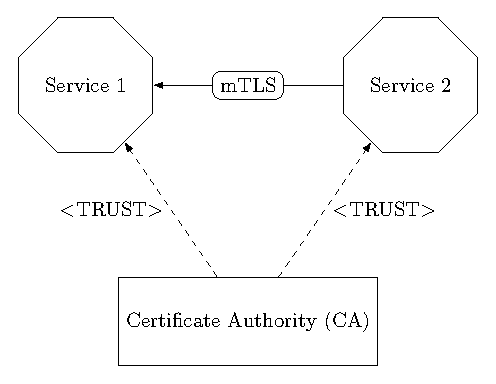
\includegraphics{images/authentication-mechanisms/TikZ_mTLS_base_structure.pdf}
	\caption{Setup using mTLS for the service-to-service authentication~\cite{dias2020microservices}}
	\label{fig:auth_mechanisms_mtls}
\end{figure}

\section{Authentication based on mTLS}
% TODO: Kurz erklären welchen Zusammenhang mtls mit Client Certificate Authentication hat
Mutual TLS is the most popular option for the service-to-service authentication of microservice deployments~\cite{dias2020microservices}.
Securing the communication with TLS already provides integrity, confidentiality and furthermore authenticates the server to the client.
Since basic TLS does not provide authentication from the client to the server, it is not sufficient for the service-to-service security.
Therefore mutual TLS is used, which provides an efficient and straightforward approach to authenticate the client to the server.

The authentication using mTLS requires a PKI, same as the authentication using basic TLS.
It is possible to use the already existing PKI of the internet, but this would make the key management much harder and would not bring any advantages.
% TODO: Insert Reference to self hosted PKI
Therefore it is good practise to use a self-hosted PKI to have a root of trust within the network~\cite{dias2020microservices}.
The setup of a microservice deployment using mTLS is shown in figure~\ref{fig:auth_mechanisms_mtls}.

When mTLS is used, both the server and the client must provide a valid certificate to create a communication channel.
The issuer of the presented certificates must be trusted by all communicating parties~\cite{dias2020microservices}.
If one communication partner does not have a valid certificate which is signed by a trusted issuer, the communication is neglected.
Therefore each service needs a private key, a public key.
Additionally a signed certificate, which binds the public key to the subject of the certificate, is needed.
The certificates of the communication partners are exchanged during the TLS handshake.

\subsection{Handshake}
\label{sec:tlshandshake_details}
The handshake is used exchange to exchange the certificates of the participants and setup the connection.
The steps of the handshake differ between the used algorithms and versions of the TLS protocol.
The following sequence and figure~\ref{fig:tlshandshake} should give an overview about the steps of the TLS handshake using mutual TLS~\cite{parsovs2013practical}:
\begin{enumerate}
	\item The client initializes the connection by sending a \textbf{ClientHello} message to the server.
		The \textbf{ClientHello} message includes a list of supported cipher suits, and the randomness, which is a combination of random bytes and the current date~\cite{mediumtls}.
	\item The sever responds with a \textbf{ServerHello}, in which the server chooses one cipher suite of the \textbf{ClientHello} message.
		Furthermore the \textbf{ServerHello} contains the servers randomness.
	\item The server sends the \textbf{Certificate} messages, containing one or more certificates, which can be used to build the chain.
		The client validates the sent certificates with his own trusted store.
		If the trusts the sent certificate chain, the server is authenticated successfully.
	\item The server sends the \textbf{CertificateRequest} message, in which the trusted CAs of the server are listed.
		The client can use this list to choose the correct certificate he has to present.
	\item The server sends the \textbf{ServerHelloDone} message.
	\item The client responds with his \textbf{Certificate} message, which is similiar to the servers \textbf{Certificate} message, but contains the client's certificate.
	\item The client he generates a random value the pre-master secret, which is used to derive symmetric keys for the cipher suite.
		The pre-master secret is then encrypted, using the public key of the server.
		The public key of the server is assumed to be the first certificate of the \textbf{Certificate} message by the server.
		The encrypted pre-master secret is then transferred to the server within the \textbf{ClientKeyExchange} message.
	\item The client has to proove the client that he owns the corresponding private key of the sent certificate.
		Therefore he has to encrypt the hash of all previous messages with his private key.
		This encrypted hash is then sent to the server within the \textbf{CertificateVerify} message.
		The sever can decrypt the hash with the public key of the certificate and can calculate the hash on his own to check whether the decrypted hash is correct or not.
	\item The client sends a \textbf{ChangeCipherSpec} message, to signal the server, that all following messages will be protected with the protection mechanisms defined in the cipher suite.
	\item The last message of the handshake is the \textbf{Finished} message, which is an encrypted hash of all previous messages.
\end{enumerate}
After the handshake both participants know the secret, which can be used to encrypt and decrypt messages.
The handshake would have almost the same steps when mTLS is not used.
Only the \textbf{CertificateRequest} message of the sever and the \textbf{Certificate} message and the \textbf{CertificateVerify} message of the client are unique for mTLS.
One special case of the handshake is, that the client responds to the \textbf{CertificateRequest} with a empty \textbf{Certificate} message.
Depending on the configuration of the server, the connection without a certificates can be allowed or the connection will be aborted~\cite{parsovs2013practical}.

\begin{figure}
    \centering
	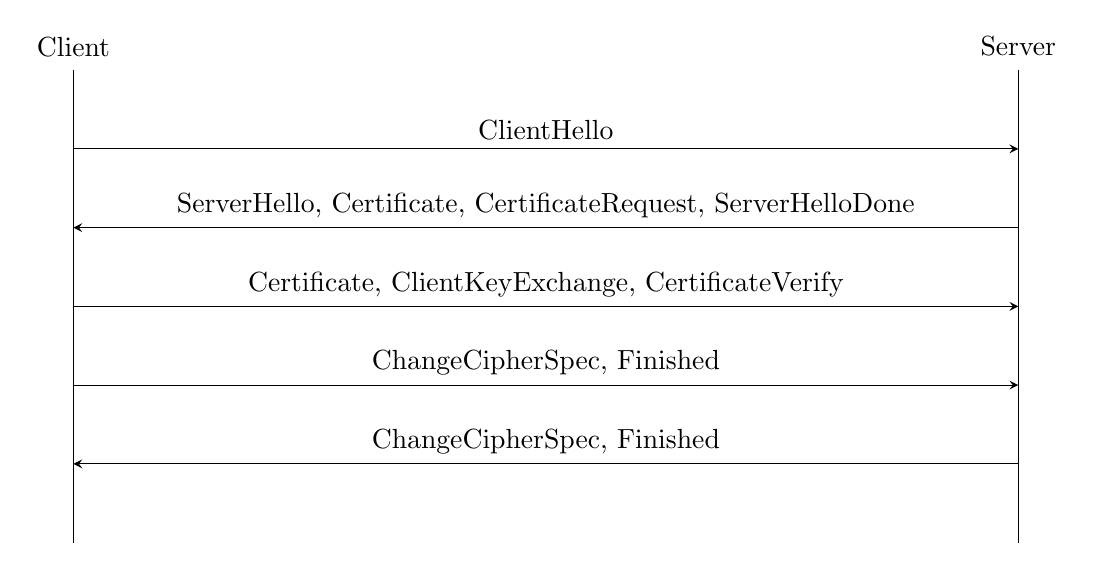
\begin{tikzpicture}
		\draw (-6,0) -- (-6,-6) (6,0) -- (6,-6);
		\node at (-6,.3) {Client};
		\node at (6,.3) {Server};

		\draw[-stealth] (-6,-1) -- node[midway,above] {ClientHello} (6,-1);
		\draw[stealth-] (-6,-2) -- node[midway,above] {ServerHello, Certificate, CertificateRequest, ServerHelloDone} (6,-2);
		\draw[-stealth] (-6,-3) -- node[midway,above] {Certificate, ClientKeyExchange, CertificateVerify} (6,-3);
		\draw[-stealth] (-6,-4) -- node[midway,above] {ChangeCipherSpec, Finished} (6,-4);
		\draw[stealth-] (-6,-5) -- node[midway,above] {ChangeCipherSpec, Finished} (6,-5);
	\end{tikzpicture}
    \caption{TLS handshake using mTLS~\cite{parsovs2013practical}}
    \label{fig:tlshandshake}
\end{figure}

\subsection{Motivation}
Mutual TLS is a very efficient mechanism to implement service to service authentication.
Usually HTTPS is used for the communication among the microservices, which means TLS is already used.
Therefore the use of mTLS does not cause much configuration overhead and no new technologies are necessary~\cite{dias2020microservices}.

One crucial advantage of the TLS handshake is that the private keys are never exchanged and the session keys are always different, due to the usage of the randomness.
This means even if an intruder is able to get the session key of a communication, he is not able to use this key for another session.
Furthermore it is not possible to retrieve any information about the private key of the communication partners with the knowledge of the session key.
This shows how secure mTLS is, even for very advanced attack~\cite{parsovs2013practical}.

From the developer perspective, mTLS does not require the developers to implement very much logic.
The service which acts as the server has to be configured to use certificate authentication.
Depending on the used technologies, this is usually done by setting a few configuration parameters in the code, or directly on the webserver.
The service which acts as the client has to be configured to send his certificate during the TLS handshake.
Most HTTP Client libraries support to simply attach the certificate to each HTTP Request.
If the Factory pattern is used, the configuration is even needed once for a entire service.

The previously mentioned motivations show, that mTLS makes service-to-service security very simple.
It is perfectly fitted for projects, which want to keep the authentication mechanism simple and efficient.
But, since it is an extension for the TLS protocol, the configuration and extension options are very limited.

\subsection{Challenges}
% TODO: Referenz auf key management
The biggest challenge of mTLS is the key management, which was described in more detail in chapter.
Key management is responsible for key provisioning, key revocation, key rotation and some more management tasks.
Usually the key management results in requiring a self-hosted PKI for the deployment.
For small applications the key management can be kept very simple.
But automation tools are required, as soon as the deployment grows and many services are running at the same time.
Therefore the management overhead of mTLS is much harder to handle, than the implementation of mTLS itself~\cite{dias2020microservices}.

The services of a microservice deployment usually host their APIs on webservers.
Since microservice deployment's have multiple technology stacks, multiple different webservers might have to be used.
The configuration of mTLS for a webserver is different from webserver to webserver.
So the configuration has to be done multiple times, which results in a bigger attack surface.
Especially because the mTLS implementations of the webservers might have bugs.
Those bugs can be very hard to fix, because the developers have to fully rely on the support of the webserver developers. 
For example the apache webserver, which is one of the most popular webservers had many issues, in combination with mTLS.
Resulting in many security risks, caused by wrong configurations~\cite{parsovs2013practical}. 


